
\section*{Stammfunktion und unbestimmtes Integral}


\subsection*{Grundintegrale (+ c jeweils weggelassen)}

\begin{tabular}{|l|l|l|}
\hline 
e / ln & sin / cos / tan & allgemein\tabularnewline
\hline 
$\int e^{x}\cdot dx=e^{x}$ & $\int sin^{2}(x)\cdot dx=\frac{x}{2}-\frac{1}{2}\cdot sin(x)\cdot cos(x)$  & $\int x^{n}\cdot dx=\frac{x^{n+1}}{n+1}+c,n\neq1$\tabularnewline
\hline 
$\int e^{-2x}=\frac{e^{-2x}}{-2}$ & $\int cos^{2}(x)\cdot dx=\frac{1}{2}(x+sin(x)\cdot cos(x))$  & $\int\frac{1}{\sqrt{a^{2}-x^{2}}}=arcsin\frac{x}{|a|}$\tabularnewline
\hline 
$\int\frac{1}{e}=\frac{x}{e}$ & $\int tan^{2}(x)=tan(x)-x$ & $\int a^{x}\cdot dx=\frac{a^{x}}{\ln(a)}+c,a>0,a\neq1$\tabularnewline
\hline 
$\int be^{ax}\cdot dx=\frac{b}{a}e^{ax}$ & $\int\frac{1}{sin(x)}=ln(sin(\frac{x}{2}))-ln(cos(\frac{x}{2}))$ & $\int e^{\ln(a)\cdot x}\cdot dx=\frac{a^{x}}{\ln(a)}+c,a>0,a\neq1$\tabularnewline
\hline 
$\int e^{-2x+1}=\frac{e^{-2x+1}}{-2}$ & $\int\frac{1}{cos(x)}=ln(sin(\frac{x}{2})+cos(\frac{x}{2}))-ln(cos(\frac{x}{2})-sin(\frac{x}{2}))$ & $\int\frac{1}{x^{2}}=-\frac{1}{x}$\tabularnewline
\hline 
$\int\frac{1}{x}\cdot dx=\ln\mid x\mid$ & $\int\frac{1}{tan(x)}=ln(sin(x))$ & $\int\frac{1}{x}\cdot dx=\ln\mid x\mid$\tabularnewline
\hline 
$\int\frac{1}{x-5}\cdot dx=\ln\mid x-5\mid$ & $\int\frac{1}{sin^{2}(x)}=-cotan(x)$ & $\int\frac{1}{x^{2}+a^{2}}\cdot dx=\frac{1}{a}\cdot arctan(\frac{x}{a})$\tabularnewline
\hline 
$\int\frac{1}{2x-5}\cdot dx=\ln\mid x-5\mid$ & $\int\frac{1}{cos^{2}(x)}=tan(x)$ & $\int\frac{1}{1+x^{2}}\cdot dx=tan^{-1}(x)$\tabularnewline
\hline 
$\int\frac{1}{e^{x}}=-e^{-x}$ & $\int\frac{1}{tan^{2}(x)}=-x-cotan(x)$ & $\int\frac{1}{1+x^{2}}\cdot dx=\frac{1}{2}(ln(x+1)-ln(1-x)$\tabularnewline
\hline 
$\int ln(x)dx=xln(x)-x$ & $\int x\cdot sin(x)\cdot dx=sin(x)-x\cdot cos(x)$  & $\int\frac{1}{\sqrt{x}}=2\sqrt{x}$\tabularnewline
\hline 
$\int x\cdot ln(x)dx=\frac{1}{4}x^{2}(2\cdot ln(x)-1)$ & $\int sin(ax)\cdot dx=-\frac{cos(ax)}{a}$  & Tipps\tabularnewline
\hline 
 & $\int x\cdot cos(x)\cdot dx=x\cdot sin(x)+cos(x)$  & $tan=\frac{sin}{cos}$\tabularnewline
\hline 
 & $\int2x\cdot cos(x)\cdot dx=2x\cdot sin(x)+2cos(x)$  & $e^{ln(x)}=x$\tabularnewline
\hline 
 & $\int\frac{sin(x)}{cos(x)}=\int tan(x)=-ln(cos(x))$ & $ln(e^{x})=x$\tabularnewline
\hline 
$u=\frac{y}{x}$ & $\int sin^{2}(ax)\cdot dx=\frac{x}{2}-\frac{sin(2ax)}{4a}$ & $u^{\frac{3}{2}}=(u^{\frac{1}{2}})^{3}=\sqrt{u}^{3}=u\cdot\sqrt{u}$\tabularnewline
\hline 
 & $\int sin(x)\cdot cos(x)\cdot dx=-\frac{1}{2}cos^{2}(x)$ & $ln(x)'=\frac{1}{x}$\tabularnewline
\hline 
 & $\int tan(x)\cdot cos(x)\cdot dx=\int sin(x)\cdot dx=-cos(x)$ & $(e^{x})'=e^{x}$\tabularnewline
\hline 
\end{tabular}

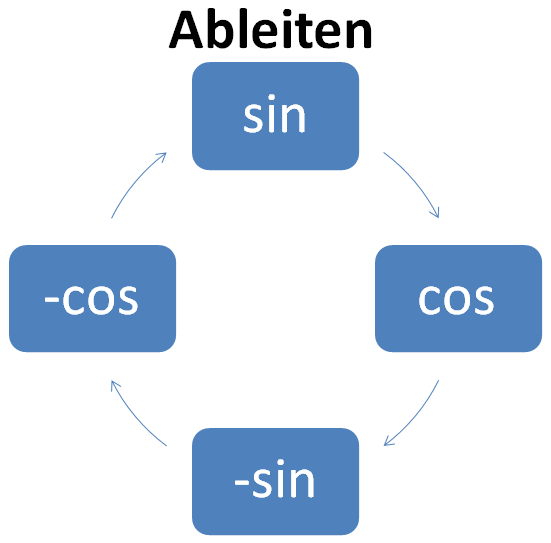
\includegraphics[width=4cm]{Integral/sin}


\subsection*{Elementare Rechenregeln}


\subsubsection*{Regel vom konstanten Faktor}

$\int k\cdot f(x)\cdot dx=k\cdot F(x)+c$
\begin{itemize}
\item $\int25e^{x}\cdot dx=25\cdot e^{x}+c$
\item $\int-13x^{3}\cdot dx=-13\cdot\frac{x^{4}}{4}+c$
\end{itemize}

\subsubsection*{Skalierungsregel}

$\int f(k\cdot x)\cdot dx=\frac{F(k\cdot x)}{k}+c$
\begin{itemize}
\item $\int e^{\frac{3}{2}x}\cdot dx=\frac{e^{\frac{3}{2}x}}{\frac{3}{2}}+c=\frac{2}{3}\cdot e^{\frac{3}{2}x}$
\end{itemize}

\subsubsection*{Translationsregel}

$\int f(x+k)\cdot dx=F(x+k)+c$
\begin{itemize}
\item $\int\frac{1}{x-6}\cdot dx=ln\mid x-6\mid+c$
\end{itemize}

\subsubsection*{Summenregel}

$\int f(x)\pm g(x)\cdot dx=F(x)\pm G(x)+c$
\begin{itemize}
\item $\int(8x^{3}-4x+2)\cdot dx=8\cdot\frac{x^{4}}{4}-4\cdot\frac{x^{2}}{2}+2x+c=2x^{4}-2x^{2}+2x+c$
\end{itemize}

\subsubsection*{Produkteregel / Partielle Integration}

$\int f(x)\cdot g(x)\cdot dx=F(x)\cdot g(x)-\int F(x)\cdot g^{\prime}(x)\cdot dx$
\begin{itemize}
\item $\int x^{2}\cdot e^{x}\cdot dx=e^{x}\cdot x^{2}-\int e^{x}\cdot2x\cdot dx=e^{x}\cdot x^{2}-2[x\cdot e^{x}-\int1\cdot e^{x}\cdot dx]=e^{x}\cdot x^{2}-2xe^{x}+2e^{x}+c=e^{x}[x^{2}-2x+2]+c$
\end{itemize}
Bemerkung: Hier wurde $x^{2}$jeweils abgeleitet und $e^{x}$integriert.
\begin{itemize}
\item $\int x\cdot cos(x)\cdot dx=sin(x)\cdot x-\int1\cdot sin(x)\cdot dx=sin(x)\cdot x+cos(x)+c$
\end{itemize}
Bemerkung: Hier wurde x abgeleitet und cos(x) integriert.


\subsection*{Integration und Substitution}
\begin{itemize}
\item $\int f(u(x))\cdot u^{\prime}\cdot dx=\int f(u)\cdot du$
\item $\int\frac{u'(x)}{u(x)}dx=\int\frac{du}{u}=ln|u|+c$
\item $\frac{dx}{du}=u^{\prime}(x)$
\end{itemize}
Trick: Zähler eines Bruches so korrigieren, das es der Ableitung der
Funktion entspricht. Anschliessend kann $u^{\prime}\cdot dx$ durch
$du$ ersetzt werden.
\begin{itemize}
\item $\int\frac{1}{(4x+5)^{3}}\cdot dx=\frac{1}{4}\cdot\int\frac{4}{(4x+5)^{3}}\cdot dx=\frac{1}{4}\cdot\int\frac{u^{\prime}}{u^{3}}\cdot dx=\frac{1}{4}\cdot\int\frac{du}{u^{3}}=\frac{1}{4}\cdot\frac{u^{-2}}{-2}+c=-\frac{1}{8u^{2}}+c=-\frac{1}{8}\cdot\frac{1}{(4x+e)^{2}}+c$
wobei $dx=\frac{du}{u}$
\item $\int\frac{x}{\sqrt{a^{2}-x^{2}}}\cdot dx=\int\frac{x}{\sqrt{u}}\cdot dx=\int\frac{x}{\sqrt{u}}\cdot\frac{du}{u^{\prime}}=\int\frac{x\cdot du}{-2x\cdot\sqrt{u}}=-\int\frac{du}{2\cdot\sqrt{u}}=-\frac{1}{2}\cdot u^{\frac{1}{2}}\cdot2+c=-\sqrt{u}+c=-\sqrt{a^{2}-x^{2}}+c$
\end{itemize}
Spezialfall:
\begin{itemize}
\item $\int\frac{u^{\prime}(x)\cdot dx}{u(x)}=\int\frac{du}{u}=ln\mid u\mid+c=ln\mid u(x)\mid+c$
\item $\int\frac{x}{4+x^{2}}\cdot dx=\frac{1}{2}\cdot\int\frac{2x}{4+x^{2}}\cdot dx=\frac{1}{2}\cdot\int\frac{du}{u}=\frac{1}{2}\cdot ln\mid u\mid+c=\frac{1}{2}\cdot ln\mid4+x^{2}\mid+c$
\end{itemize}

\subsection*{Partialbruchzerlegung}

Wird gebraucht um gebrochenrationale Funktionen zu integrieren:
\begin{verse}
$\int\frac{p(x)}{q(x)}\cdot dx$
\end{verse}
Man unterscheidet:
\begin{itemize}
\item Grad Zähler$\geq$Grad Nenner = unechtgebrochen
\item Grad Zähler < Grad Nenner = echtgebrochen
\end{itemize}

\subsubsection*{Unechtgebrochen}

Mit Hilfe der Polynomdivision lassen sich solche Quotienten zerlegen
in ein Polynom und in einen echtgebrochenen Quotienten


\subsubsection*{Echtgebrochen}

Grundsätzlich muss man das Polynom in Faktoren zerlegen die höchstens
quadratisch sind.


\paragraph*{1. Fall}

q(x) zerfällt in verschiedene lineare Faktoren (hat m einfache Nullstellen):
\begin{itemize}
\item $q(x)=x^{2}-4x+3=(x-1)(x-3)$
\end{itemize}
Ansatz:
\begin{itemize}
\item $\int\frac{p(x)}{q(x)}=\int\frac{A_{1}}{(x-x_{1})}\cdot dx+\int\frac{A_{2}}{(x-x_{2})}\cdot dx+...+\int\frac{A_{m}}{(x-x_{m})}\cdot dx$
\item $\int\frac{3x-5}{x^{2}+2x-8}\cdot dx=\int\frac{A}{(x-2)}\cdot dx+\int\frac{B}{(x+4)}\cdot dx$
\item $\frac{3x-5}{x^{2}+2x-8}=\frac{A}{(x-2)}+\frac{B}{(x+4)}$ $\mid\cdot(x-2)\cdot(x+4)$
\item $3x-5=A(x+4)+B(x-2)$ $\mid$x einsetzen und A, B ausrechnen (z.B.
x=-4, x=2)
\item $A=\frac{1}{6};B=\frac{17}{6}$
\item $\int\frac{3x-5}{x^{2}+2x-8}\cdot dx=\frac{1}{6}\cdot\int\frac{1}{(x-2)}\cdot dx+\frac{17}{6}\cdot\int\frac{1}{(x+4)}\cdot dx=\frac{1}{6}\cdot ln\mid x-2\mid+\frac{17}{6}\cdot ln\mid x+4\mid+C$
\end{itemize}

\paragraph*{2. Fall}

q(x) zerfällt in lineare Faktoren, es gibt mindestens einen Faktor,
der mehrfach vorkommt:
\begin{itemize}
\item $q(x)=x^{3}-3x^{2}-9x-5=(x+1)^{2}\cdot(x-5)$
\end{itemize}
Ansatz:
\begin{itemize}
\item $\int\frac{p(x)}{q(x)}=\int\frac{A_{1}}{(x-x_{i})}\cdot dx+\int\frac{A_{2}}{(x-x_{i})^{2}}\cdot dx+...+\int\frac{A_{k}}{(x-x_{i})^{k}}\cdot dx$
\item $\int\frac{x^{2}+15x+8}{x^{3}-3x^{2}-9x-5}\cdot dx=\int\frac{A}{(x+1)}\cdot dx+\int\frac{B}{(x+1)^{2}}\cdot dx+\int\frac{C}{(x-5)}\cdot dx$
\item $\frac{x^{2}+15x+8}{x^{3}-3x^{2}-9x-5}=\frac{A}{(x+1)}+\frac{B}{(x+1)^{2}}+\frac{C}{(x-5)}$
$\mid\cdot(x+1)^{2}\cdot(x-5)$
\item $x^{2}+15x+8=A(x+1)(x-5)+B(x-5)+C(x-5)(x+1)^{2}$ $\mid$x einsetzen
und A, B, C ausrechnen (z.B. x=-1, x=5)
\item $A=-2;B=1;C=3$
\item $\int\frac{x^{2}+15x+8}{x^{3}-3x^{2}-9x-5}\cdot dx=-2\int\frac{1}{(x+1)}\cdot dx+1\int\frac{1}{(x+1)^{2}}\cdot dx+3\int\frac{1}{(x-5)}\cdot dx=-2\cdot ln\mid x+1\mid+\frac{(x+1)^{-1}}{-1}+3\cdot ln\mid x-5\mid+C$
\end{itemize}

\paragraph*{3. Fall}

Der Nenner enthalte quadr. Faktoren die sich nicht zerlegen lassen:
\begin{itemize}
\item $q(x)=x^{3}-6x^{2}+10x=x\cdot(x^{2}-6x+10)$
\end{itemize}
Ansatz:
\begin{itemize}
\item $\int\frac{p(x)}{q(x)}=\int\frac{B_{1}x+C_{1}}{Q(x)^{1}}\cdot dx+\int\frac{B_{2}x+C_{2}}{Q(x)^{2}}\cdot dx+...+\int\frac{B_{k}x+C_{k}}{Q(x)^{k}}\cdot dx$
\item $\int\frac{7x^{2}-19x+30}{x^{3}-6x^{2}+10x}\cdot dx=\int\frac{A}{x}\cdot dx+\int\frac{Bx+C}{x^{2}-6x+10}\cdot dx$
\item $\frac{7x^{2}-19x+30}{x^{3}-6x^{2}+10x}=\frac{A}{x}+\frac{Bx+C}{x^{2}-6x+10}$
$\mid\cdot x\cdot(x^{2}-6x+10)$
\item $7x^{2}-19x+30=A(x^{2}-6x+10)+x\cdot(Bx+C)$ $\mid$x einsetzen und
A, B, C ausrechnen (z.B. x=0,x=1, x=-1)
\item $A=3;B=4;C=-1$
\item $\int\frac{7x^{2}-19x+30}{x^{3}-6x^{2}+10x}\cdot dx=3\cdot\int\frac{1}{x}\cdot dx+\int\frac{4x-1}{x^{2}-6x+10}\cdot dx=3\cdot ln\mid x\mid+(*)$

\begin{itemize}
\item $(x^{2}-6x+10)^{\prime}=2x-6\Rightarrow4x-1=2\cdot(2x-6)+11$
\end{itemize}
\item $(*)=\int\frac{2(2x-6)+11}{x^{2}-6x+10}\cdot dx=2\cdot\int\frac{2x-6}{x^{2}-6x+10}\cdot dx+\int\frac{11}{x^{2}-6x+10}\cdot dx$

\begin{itemize}
\item $(1)=2\cdot\int\frac{2x-6}{x^{2}-6x+10}\cdot dx=2\cdot\int\frac{du}{u}\cdot dx=2\cdot ln\mid u\mid=2\cdot ln\mid x^{2}-6x+10\mid$
\item $(2)=11\cdot\int\frac{1}{x^{2}-6x+10}\cdot dx=11\cdot\int\frac{1}{(x-3)^{2}+1}\cdot dx$
ist von der Form $k\cdot\int\frac{1}{(x-C)^{2}+a^{2}}\cdot dx$
\item $=k\cdot\frac{1}{a}\cdot arctan(\frac{x-C}{a})+C=11\cdot\frac{1}{1}\cdot arctan(\frac{x-3}{1})+C$
\end{itemize}
\item $\int f(x)\cdot dx=3\cdot ln\mid x\mid+2\cdot ln\mid x^{2}-6x+10\mid+11\cdot arctan(x-3)+C$
\end{itemize}

\section*{Das bestimmte Integral}


\subsection*{Das Flächenproblem}

$\underset{a}{\overset{b}{\int}}f(x)\cdot dx=A$
\begin{enumerate}
\item Zwischenwerte $x_{0},x_{1},...,x_{n}$setzen und somit Intervall {[}a,b{]}
in Teilintervalle zerlegen.
\item Wähle in jedem Teilintervall eine Zwischenstelle $\xi_{i}$

\begin{enumerate}
\item $A_{1}=\Delta x\cdot f(\xi_{1})$
\item $A_{k}=\Delta x\cdot f(\xi_{k})$
\end{enumerate}
\item $S_{n}=A_{1}+...+A_{n}=\overset{n}{\underset{k=1}{\sum}}A_{k}=\overset{n}{\underset{k=1}{\sum}}\Delta x\cdot f(\xi_{k})$
\item Grenzübergang: $\underset{n\rightarrow\infty}{lim}S_{n}=A\Rightarrow(\Delta x\rightarrow0)$
\end{enumerate}

\paragraph*{Riemannsche Summen}

$\intop_{a}^{b}f(x)dx:=lim_{n\rightarrow\infty(\triangle x\rightarrow0)}\sum_{i=1}^{n}f(\xi_{i})\times\Delta x_{i}$


\subsection*{Exakt mit Grenzübergang}
\begin{verse}
$f(x)=x^{2}$
\end{verse}
Teile Intervall {[}0,2{]} in n gleiche Teile:
\begin{verse}
\begin{tabular}{|c|c|c|c|c|cl}
\cline{1-5} 
Intervall & Breite &  & Höhe & Fläche &  & Vorgehen\tabularnewline
\cline{1-5} \cline{7-7} 
$I_{1}=[0\cdot\frac{2}{n},1\cdot\frac{2}{n}]$ & $\Delta x_{1}=\frac{2}{n}$ & $\xi_{1}=1\cdot\frac{2}{n}$ & $f(\xi_{1})=(1\cdot\frac{2}{n})^{2}$ & $A_{1}=\frac{2}{n}\cdot1^{2}\cdot\frac{4}{n^{2}}$ &  & - allgemeines Intervall\tabularnewline
\cline{1-5} 
$I_{2}=[1\cdot\frac{2}{n},2\cdot\frac{2}{n}]$ & $\Delta x_{2}=\frac{2}{n}$ & $\xi_{2}=2\cdot\frac{2}{n}$ & $f(\xi_{2})=(2\cdot\frac{2}{n})^{2}$ & $A_{2}=\frac{2}{n}\cdot2^{2}\cdot\frac{4}{n^{2}}$ &  & - Auswertungsstelle {]} Wert an AS\tabularnewline
\cline{1-5} 
$I_{k}=[(k-1)\cdot\frac{2}{n},k\cdot\frac{2}{n}]$ & $\Delta x_{k}=\frac{2}{n}$ & $\xi_{k}=k\cdot\frac{2}{n}$ & $f(\xi_{k})=(k\cdot\frac{2}{n})^{2}$ & $A_{n}=\frac{2}{n}\cdot n^{2}\cdot\frac{4}{n^{2}}$ &  & - Flächenformel\tabularnewline
\cline{1-5} 
$I_{n}=[(n-1)\cdot\frac{2}{n},n\cdot\frac{2}{n}]$ & $\Delta x_{n}=\frac{2}{n}$ & $\xi_{n}=n\cdot\frac{2}{n}$ & $f(\xi_{n})=(n\cdot\frac{2}{n})^{2}$ & $A_{k}=\frac{2}{n}\cdot k^{2}\cdot\frac{4}{n^{2}}$ &  & - $\sum$ bilden\tabularnewline
\cline{1-5} 
\end{tabular}
\end{verse}
$S_{n}=\frac{2}{n}\cdot\frac{4}{n^{2}}\cdot\overset{n}{\underset{k=1}{\sum}}k^{2}=\frac{8}{n^{3}}\cdot\frac{n(n+1)(2n+1)}{6}=\frac{16}{6}=\frac{8}{3}$
